\section{Background} \label{backgorund}



\subsection{Stable Diffusion}
Stable Diffusion is based on a special type of Diffusion Model called Latent Diffusion Model (LDM) \cite{Rombach_2022_CVPR}. LDMs are trained to create a desired image by repeatedly denoising an image initialised with random gaussian noise. What separates LDMs from regular Diffusion Models is that they apply the diffusion process in a lower-dimensional latent space instead of the pixel-space. This greatly alleviates the need for extensive resources, especially when generating larger images. LDMs have three main components: 1) the autoencoder, 2) the U-Net and 3) the text-encoder.
\begin{figure}[!htb]
\centering
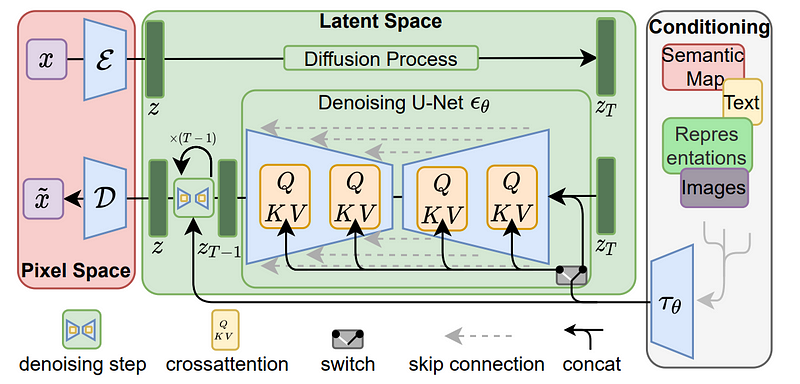
\includegraphics[width=0.8\textwidth]
{static/LDM.png}
\caption{The LDM \cite[Fig.~3]{Rombach_2022_CVPR}.}
\label{fig:ldm}
\end{figure}



\subsubsection{The Autoencoder}
A Variational Autoencoder (VAE) consists of two parts: the encoder and the decoder. "During latent diffusion training, the encoder is used to get the latent representations (latents) of the images for the forward diffusion process, which applies more and more noise at each step" \cite{patil2022stable}. The decoder conversely transforms the denoised latents, created by the U-Net, back into the pixel space at the end of the diffusion process. Only the decoder is used for the image generation process (see Fig.~\ref{fig:ldm}).



\subsubsection{The U-Net}
The U-Net \cite{ronneberger2015u} is a type of Convolutional Neural Network (CNN) that is responsible for predicting the noise in the current sample image. The image generation process starts with a random sample image of gaussian noise. The U-Net then takes this sample \((latents)\) and predicts the noise residual \((noise\_pred)\) of the image. 
This noise residual is partially \((sigma)\) removed in every step, until we end up with the final fully denoised image (see Fig.~\ref{fig:ldm}).
\begin{lstlisting}[language=Python]
latens = latents - sigma * noise_pred
\end{lstlisting}
The U-Net consists of an encoder and a decoder with transformer-based blocks. "Thus, it first encodes the current noised image as a set of tokens, then passes it through a series of transformer blocks" \cite{bolya2023tomesd}. The inclusion of transformer-based blocks allows the model to not only preserve the spacial hierarchies but also the semantic structure of the image.\\
A further aspect that distinguishes the U-Net from an autoencoder are the skip connections that directly pass information from the encoder to the decoder, aiding in the preservation of details during upsampling (see Fig.~\ref{fig:ldm}).



\subsubsection{The Text-Encoder}
The text-encoder is a transformer-based encoder that converts the input prompt from a string to an embedding vector that captures the semantic meaning of text and can be interpreted by the U-Net. Stable Diffusion uses CLIP's \cite{radford2021learning} pre-trained text-encoder \href{https://huggingface.co/docs/transformers/model_doc/clip#transformers.CLIPTextModel}{CLIPTextModel} and thus avoids additional training of the text-encoder.



\subsubsection{The Transformer Block}
Every transformer block has a self-attention (self-attn), cross-attention (cross-attn) and multi-layer perceptron (mlp) module.
The transformer also has residual connections around these modules to preserve important information and improve gradient flow, as well as multiple layer normalization blocks.



\subsubsection*{Self-Attention}
Self-attention \cite{vaswani2017attention} takes a series of (token) vectors and computes outputs while attending to every other token in the sequence.\\
The input vectors \((X)\) are firstly transformed into three different embedding matrices called Queries \((Q)\), Keys \((K)\) and Values \((V)\),  by multiplying the inputs with special transformation matrices \((W_Q, W_K, W_V)\). Then the self-attention module computes the attention weights \((A)\) for every pair of input vectors by taking the scaled dot-product of the Query and Key matrix and then applying the softmax-function. Lastly, the output vectors \((Y)\) are generated by taking a weighted sum of the Value embeddings with the attention weights (see Fig.~\ref{fig:self-attn}).\\
The output vectors are transformed representations of the input vectors, considering their interactions with every other input vector. The outputs are then passed on to the subsequent layers of the transformer. Self-attention enables the transformer to capture global dependencies in images or text.
\begin{figure}[!htb]
\centering
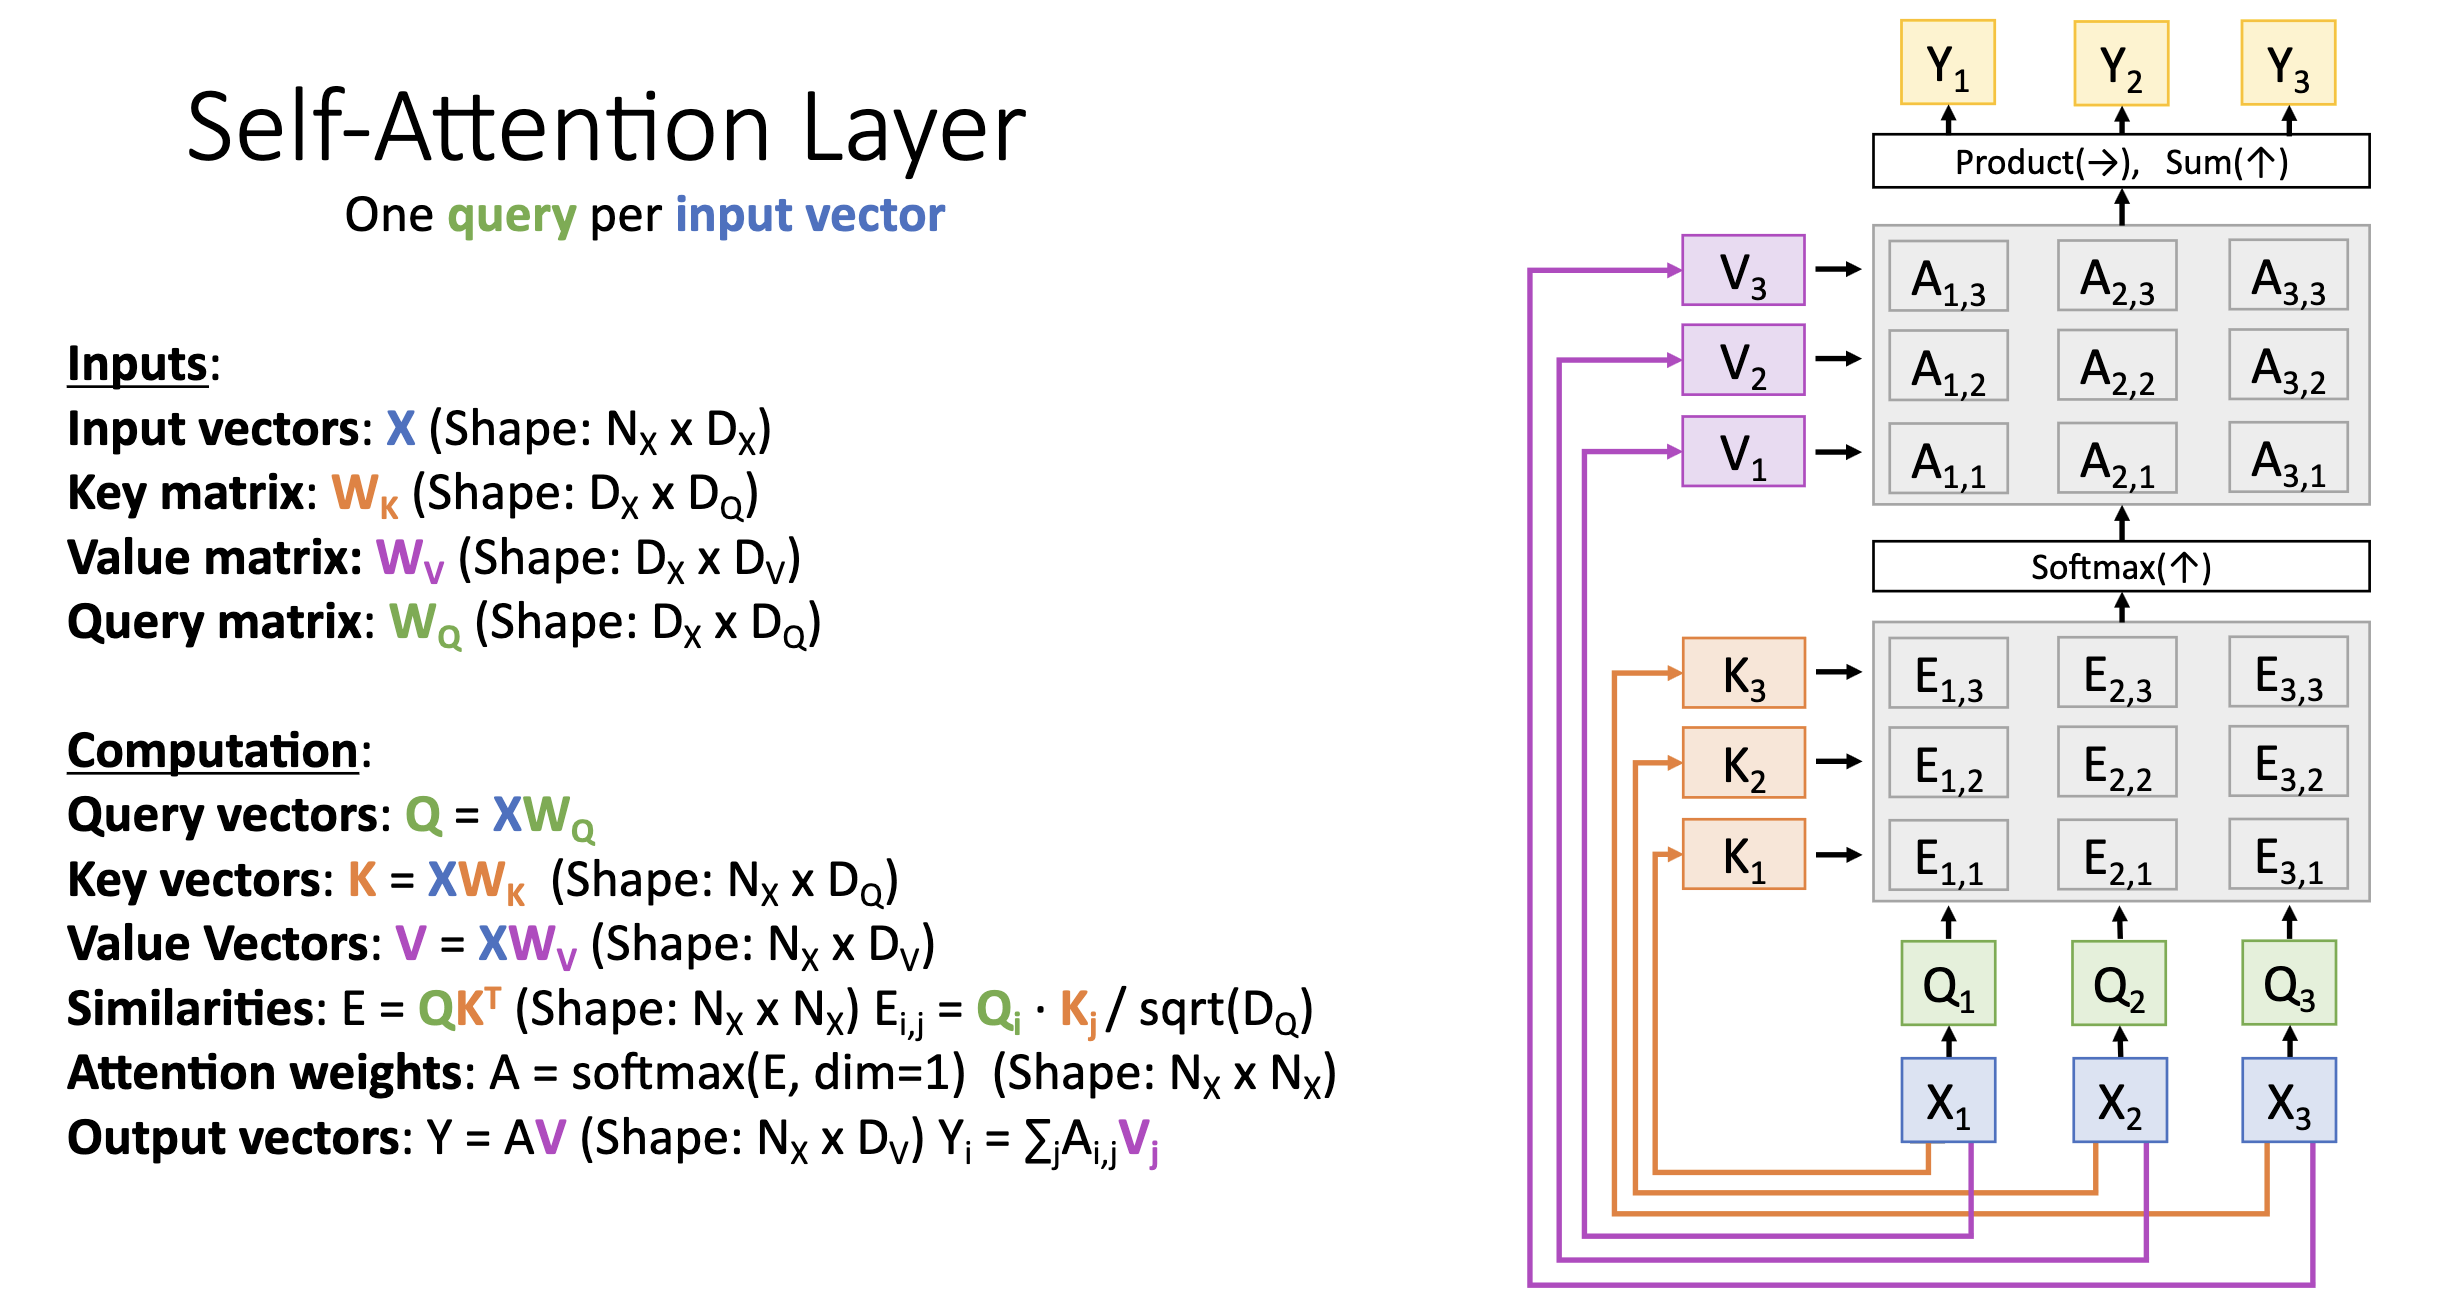
\includegraphics[width=0.95\textwidth]
{static/self_attn.png}
\caption{Self-attention \cite{johnson2019attn}}
\label{fig:self-attn}
\end{figure}



\subsubsection*{Cross-Attention}
Cross-attention creates its output from two input embeddings \((X_1, X_2)\) by generating \(Q\) from one input \((Q=X_1W_Q)\), and 
\(K\) and \(V\) from the other \((K=X_2W_K,\ V=X_2W_V)\). The algorithm is identical to self-attention from this point onwards.\\ Cross-Attention allows the model to consider both visual and semantic information when generating sequences, which enables the U-Net to attend to both the image and the prompt at the same time.



\subsubsection*{Multi-Layer Perceptron}
A multi-layer perceptron is a fully connected neural network. The mlp layer takes the outputs of the previous layer and applies an mlp network to each vector independently. This network consists of two linear transformations with a non-linear activation function (e.g., GELU \cite{hendrycks2016gaussian}) in between. Non-linearity exists exclusively in the mlp layer, allowing the transformer to capture more complex patterns in the data. It is particularly effective at modeling short-range patterns and local dependencies within a sequence.



\subsection{Fréchet-Inception-Distance}
The Fréchet Inception Distance (FID) is a metric that is used to evaluate the quality of generated images. It provides a quantitative measure of similarity by calculating the distance between the distributions of feature vectors of two image datasets. The feature vectors are extracted from the Inception model and the mean and covariance of their distributions are calculated.\\
"We call the Fréchet distance \(d(., .)\)
between the Gaussian with mean \((m, C)\) obtained from \(p(.)\) and the Gaussian with mean \((m_w, C_w)\)
obtained from \(p_w(.)\) the “Fréchet Inception Distance” (FID), which is given by:
\begin{align*}
    d^2((m,C),(m_w,C_w)) = || m - m_w ||_2^2 + Tr(C+C_w-2(CC_w)^\frac{1}{2})" 
\end{align*}
\cite{heusel2017gans}.\\
A lower FID value indicates greater similarity between the two image sets.



\subsubsection{Inception Model}
The Inception model \cite{Szegedy_2015_CVPR} is a deep convolutional neural network developed by Google researchers that is pretrained on ImageNet \cite{deng2009imagenet}. The model improves performance and efficiency in image classification and computer vision tasks by using multiple convolutional filter operations at different scales within the same layer.\\
The Inception model is used in the context of FID for creating low-dimensional latent representations of the input images, utilizing its ability to capture meaningful image features.
Current code implementations such as \cite{Seitzer2020FID} use the model's third iteration Inception-v3 \cite{szegedy2016rethinking}.



\subsubsection{Caveats}
FID is statistically biased, with its bias growing inversely proportional to the size of the image set, and the bias also depending on the model used for feature extraction \cite{Chong_2020_CVPR}. This makes comparing specific FID values from different experiments impossible, when identical sample sizes or the use of the same model are not guaranteed.\\
A further limitation of FID is the Inception model's compression of images to $299 \times 299$ pixels \cite{szegedy2016rethinking}. Thus, assessing the quality of larger images is additionally hindered as information about the images is lost by the compression.



\subsection{What are Tokens?}
Tokens are semantic units that can be processed by transformer-based models such as Stable Diffusion. Text, such as the prompt in image generation, is tokenized into words or subwords, which are then mapped to an embedding vector by the text-encoder. Image tokens capture discrete representations of their specific visual elements, with each token encoding a certain aspect of the image, such as a particular object, texture, color, or spatial region. This breakdown into smaller units is necessary for efficient computations and memory management, additionally enabling these algorithms to better capture patterns and relationships within the data.